\documentclass[doublecol]{../macros/epl2} 
% or \documentclass[page-classic]{epl2} for one column style

\title{Luminosity independent measurements of total, elastic and inelastic cross-sections at $\sqrt s = 7\,\rm TeV$}
%\shorttitle{Title} %Insert here a short version of the title if it exceeds 70 characters

\author{
The TOTEM Collaboration -- !! PRELIMINARY !!\\
G.~Antchev\thanks{INRNE-BAS, Institute for Nuclear Research and Nuclear Energy, Bulgarian Academy of Sciences, Sofia, Bulgaria.}\addtocounter{footnote}{-1}
%\addtocounter{footnote}
\and P.~Aspell\inst{8}
\and I.~Atanassov\inst{8}\hspace{-0.15cm}\footnotemark
\and V.~Avati\inst{8}
\and J.~Baechler\inst{8}
\and V.~Berardi\inst{5b,5a}
\and M.~Berretti\inst{7b}
\and E.~Bossini\inst{7b}
\and M.~Bozzo\inst{6b,6a}
\and P.~Brogi\inst{7b}
\and E.~Br\"{u}cken\inst{3a,3b}
\and A.~Buzzo\inst{6a}
\and F.~S.~Cafagna\inst{5a}
\and M.~Calicchio\inst{5b,5a}
\and M.~G.~Catanesi\inst{5a}
\and C.~Covault\inst{9}
\and M.~Csan\'{a}d\inst{4}
\and T.~Cs\"{o}rg\H{o}\inst{4}
\and M.~Deile\inst{8}
 \and K.~Eggert\inst{9}
 \and V.~Eremin\thanks{Ioffe Physical - Technical Institute of Russian Academy of Sciences.}
 \and R.~Ferretti\inst{6a,6b}
 \and F.~Ferro\inst{6a}
 \and A. Fiergolski\thanks{Warsaw University of Technology, Poland.}
 \and F.~Garcia\inst{3a}
 \and S.~Giani\inst{8}
 \and V.~Greco\inst{7b,8}
 \and L.~Grzanka\inst{8}\hspace{-0.15cm}\thanks{Institute of Nuclear Physics, Polish Academy of Science, Cracow, Poland.}\addtocounter{footnote}{-2}
 \and J.~Heino\inst{3a}
 \and T.~Hilden\inst{3a,3b}
 \and M.~R.~Intonti\inst{5a}
%\and M.~Janda\inst{1b}
 \and J.~Ka\v{s}par\inst{1a,8}
 \and J.~Kopal\inst{1a,8}
 \and V.~Kundr\'{a}t\inst{1a}
 \and K.~Kurvinen\inst{3a}
 \and S.~Lami\inst{7a}
 \and G.~Latino\inst{7b}
 \and R.~Lauhakangas\inst{3a}
 \and  T.~Leszko\footnotemark
 %\thanks{Warsaw University of Technology, Poland}
 \and E.~Lippmaa\inst{2}
 \and M.~Lokaj\'{\i}\v{c}ek\inst{1a}
 \and M.~Lo~Vetere\inst{6b,6a}
 \and F.~Lucas~Rodr\'{i}guez\inst{8}
 \and M.~Macr\'{\i}\inst{6a}
 \and L.~Magaletti\inst{5b,5a}
%\and G.~Magazz\`{u}\inst{7a}
 \and T.~M\"aki\inst{3a}
 \and A.~Mercadante\inst{5b,5a}
%\and M.~Meucci\inst7b
 \and N.~Minafra\inst{8} 
 \and S.~Minutoli\inst{6a}\addtocounter{footnote}{1}
 \and F.~Nemes\inst{4}\hspace{-0.15cm}\thanks{Department of Atomic Physics, ELTE University, Hungary.}
 \and H.~Niewiadomski\inst{8}
%\and E.~Noschis\inst{8}
%\and T.~Nov\'{a}k\inst{4}\thanks{KRF,  Gy\"{o}ngy\"{o}s, Hungary}
 \and E.~Oliveri\inst{7b}
 \and F.~Oljemark\inst{3a,3b}
 \and R.~Orava\inst{3a,3b}
 \and M.~Oriunno\inst{8}\hspace{-0.15cm}\thanks{SLAC National Accelerator Laboratory, Stanford CA, USA.}
 \and K.~\"{O}sterberg\inst{3a,3b}
 \and P.~Palazzi\inst{7b}
 \and J.~Proch\'{a}zka\inst{1a}
 \and M.~Quinto\inst{5a}
 \and E.~Radermacher\inst{8}
 \and E.~Radicioni\inst{5a}
 \and F.~Ravotti\inst{8}
 \and E.~Robutti\inst{6a}
 \and L.~Ropelewski\inst{8}
 \and G.~Ruggiero\inst{8}
 \and H.~Saarikko\inst{3a,3b}
% \and G.~Sanguinetti\inst{7a}
 \and A.~Santroni\inst{6b,6a}
 \and A.~Scribano\inst{7b}
 \and W.~Snoeys\inst{8}
 \and J.~Sziklai\inst{4}
 \and C.~Taylor\inst{9}
 \and N.~Turini\inst{7b}
 \and V.~Vacek\inst{1b}
 \and M.~Vitek\inst{1b}
 \and J.~Welti\inst{3a,3b}
 \and J.~Whitmore\inst{10}
 }          %ends author list
\shortauthor{The TOTEM Collaboration (G.~Antchev \etal)}
%\vspace{0.5cm}
\institute{
\inst{1a}{Institute of Physics of the Academy of Sciences of the Czech Republic, Praha, Czech Republic.}\\
\inst{1b}{Czech Technical University, Praha, Czech Republic.}\\
\inst{2} {National Institute of Chemical Physics and Biophysics NICPB, Tallinn, Estonia.}\\
\inst{3a}{Helsinki Institute of Physics, Finland.}\\
\inst{3b}{Department of Physics, University of Helsinki, Finland.}\\
\inst{4} {MTA Wigner Research Center, RMKI, Budapest, Hungary.}\\
\inst{5a}{INFN Sezione di Bari, Italy.}\\
\inst{5b}{Dipartimento Interateneo di Fisica di Bari, Italy.}\\
\inst{6a}{Sezione INFN, Genova, Italy.}\\
\inst{6b}{Universit\`{a} degli Studi di Genova, Italy.}\\
\inst{7a}{INFN Sezione di Pisa, Italy.}\\
\inst{7b}{Universit\`{a} degli Studi di Siena and Gruppo Collegato INFN di Siena, Italy.}\\
\inst{8} {CERN, Geneva, Switzerland.}\\
\inst{9} {Case Western Reserve University, Dept. of Physics, Cleveland, OH, USA.}\\
\inst{10}{Penn State University, Dept. of Physics, University Park, PA, USA.}\\
}


\pacs{13.60.Hb}{Total and inclusive cross sections (including deep-inelastic processes)}


\abstract{%
!! THIS IS JUST A PLACEHOLDER !!\\
TOTEM has measured the differential cross-section for elastic proton-proton scattering
at the LHC energy of √
s = 7 TeV analysing data from a short run with dedicated large-β∗ optics.
A single exponential fit with a slope B = (20.1 0.2stat 0.3syst ) GeV−2 describes the range of the
± ±four-momentum transfer squared from 0.02 to 0.33 GeV2. After the extrapolation to = 0,
|t| |t|a total elastic scattering cross-section of (24.8 0.2stat 1.2syst) mb was obtained. Applying
± ±the optical theorem and using the luminosity measurement from CMS, a total proton-proton
cross-section of (98.3 0.2stat 2.8syst) mb was deduced which is in good agreement with the
± ±expectation from the overall fit of previously measured data over a large range of center-of-mass
energies. From the total and elastic pp cross-section measurements, an inelastic pp cross-section
of (73.5 0.6stat +1.8
 syst) mb was inferred.
± −1.3
}


\def\d{{\rm d}}
\def\un#1{\,{\rm #1}}
\def\ung#1{\quad[{\rm #1}]}
\def\unt#1{[{\rm #1}]}
\def\e{{\rm e}}

\setbox123\hbox{$0$}
\setbox124\hbox{$.$}
\def\S{\hbox to\wd123{\hss}}
\def\.{\hbox to\wd124{\hss}}


\begin{document}

\maketitle

%--------------------------------------------------
\section{Introduction}


The papers \cite{epl96} and \cite{P1} presented two analyses of $\rm pp$ elastic scattering, determining the integral elastic cross-section $\sigma_{\rm el}$ and the intercept of the differential cross-section $\d\sigma_{\rm el}/\d t|_{0}$. These quantities can be related to the total cross-section $\sigma_{\rm tot}$ and the inelatic cross-section $\sigma_{\rm inel}$ via the optical theorem:
\begin{equation}
\label{eq:m el}
	\sigma_{\rm tot}^2 = {16\pi\, (\hbar c)^2\over 1 + \rho^2}\, \left. \d\sigma_{\rm el}\over\d t\right|_0\ ,\qquad
	\sigma_{\rm inel} = \sigma_{\rm tot} - \sigma_{\rm el}\ .
\end{equation}
The results for the low-luminosity measurement \cite{epl96} and the higher-luminosity measurement \cite{P1} are summarized in Tab.~\ref{tab:cs}.

For the $\rho$ parameter in Eq.~(\ref{eq:m el}) (the ratio of the real to the imaginary of the forward hadronic scattering amplitude), the COMPETE extrapolation \cite{compete} was used. Since this is only an extrapolation, a $\rho$-independent cross-sections will be presented and the value of $\rho$ will be constrained too.

In the paper \cite{P2}, the inelastic cross-section was determined from the same dataset as the elastic measurements in paper \cite{P1}. This enables for deriving further quantities, which is the subject of this paper. The elastic and inelastic measurements can be combined in several ways, each time eliminating some of the uncertainty factors ($\rho$, luminosity, etc.).

This paper is mostly based on the data collected in a run in October 2011. That run was split into three datasets with Roman Pot detectors at different positions (for details see Tab.~1 in \cite{P1}). All calculations were done independently for these three datasets, showing an excellent match. Therefore only the results for the three datasets combined will be given below. For completeness, some of the results will be compared to those of \cite{epl96}, obtained from a run from June 2011, where only the elastic part of the analysis could be performed.


%--------------------------------------------------
\section{$\rho$-independent quantities}

Summing the elastic cross-section from \cite{P1} and the inelastic cross-section from \cite{P2} yields total cross-section
\begin{equation}
\label{eq:m rho indep}
\sigma_{\rm tot} = \sigma_{\rm el} + \sigma_{\rm inel}
\end{equation}
which is manifestly $\rho$-independent. It evaluates to $\sigma_{\rm tot} = (99.1 \pm 4.3)\un{mb}$ (for details on the uncertainty composition see Tab.~\ref{tab:cs}). Apart from that, one can determine cross-section ratios which are moreover independent from the luminosity uncertainty: $\sigma_{\rm el} / \sigma_{\rm inel} = 0.345 \pm 0.009$ and $\sigma_{\rm el} / \sigma_{\rm tot} = 0.257 \pm 0.005$. TODO: link to the conclusion/interpretation


%--------------------------------------------------
\section{Luminosity independent cross-sections}

Using the optical theorem, one can combine the elastic measurements from \cite{P1} and the inelastic measurements from \cite{P2} to derive the total cross-section that is independent from the luminosity:
\begin{equation}
\label{eq:m lumi indep}
	\sigma_{\rm tot} = {16\pi\, (\hbar c)^2\over 1 + \rho^2}\, {\d N_{\rm el}/\d t|_0 \over N_{\rm el} + N_{\rm inel} }\ .
\end{equation}
Taking the COMPETE \cite{compete} preferred-model extrapolation $\rho = 0.141\pm 0.007$ yields $\sigma_{\rm tot} = (98.0 \pm 2.5)\un{mb}$.

One can use the luminosity-independent ratio $\sigma_{\rm el} / \sigma_{\rm inel}$ from the previous section to calculate the luminosity-independent $\sigma_{\rm inel} = (72.9 \pm 1.5)\un{mb}$ and $\sigma_{\rm el} = (25.1 \pm 1.1)\un{mb}$. All these cross-section values and their uncertainty compositions are summarized in Tab.~\ref{tab:cs}. TODO: ref to figure \ref{fig:cs}?


\begin{figure*}
\begin{center}
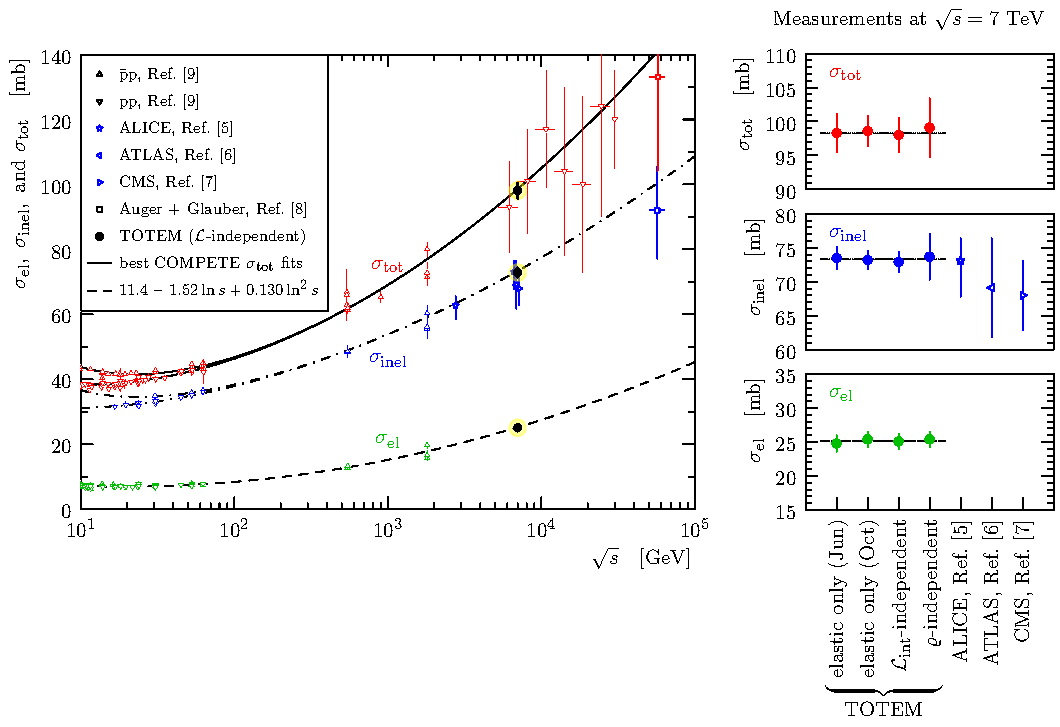
\includegraphics[width=18cm]{fig/sigma_tot_el_inel_cmp_big.pdf}
%\vskip-5mm
\caption{TODO: do we want this figure?}
\label{fig:cs}
\end{center}
\end{figure*}



\begin{largetable}
\caption{Cross-section summary. Only systematic uncertainties are indicated, the statistical uncertainties are negligible. Several uncertainty contributions are given: el (from the elastic-scattering analysis), inel (from the inelastic-scattering analysis), ${\cal L}_{\rm int}$ (from the $4\%$ uncertainty of the CMS luminosity measurement) and tot (the total uncertainty).
The $\rho$-uncertainties follow from the COMPETE preferred-model extrapolation $\rho = 0.141\pm 0.007$.}
\label{tab:cs}
\small
\setlength{\tabcolsep}{1pt}
\def\ColSep{15pt}
\begin{tabular}{cc@{\hskip\ColSep}rl @{\hskip\ColSep}cccc@{$\Rightarrow$}c @{\hskip\ColSep}cccc@{$\Rightarrow$}c @{\hskip\ColSep}cccc@{$\Rightarrow$}c}
%&\multispan{17}\hrulefill\cr
\hline
&&\multispan2\hss elastic only (Eq.~(\ref{eq:m el})) \hss &\multispan5\hss elastic only (Eq.~(\ref{eq:m el}))\hss &\multispan5\hss $\rho$-independent (Eq.~(\ref{eq:m rho indep}))\hss &\multispan5\hss ${\cal L}_{\rm int}$-independent (Eq.~(\ref{eq:m lumi indep}))\hss\cr
&&\multispan2\hss June 2011, Ref.~\cite{epl96} \hss &\multispan5\hss October 2011, Ref.~\cite{P1}\hss &\multispan5\hss October 2011\hss &\multispan5\hss October 2011\hss\cr\hline
&&& tot &&    el & $\cal L_{\rm int}$ & $\rho$ & tot &&    el & inel & $\cal L_{\rm int}$ & tot &&    el & inel & $\rho$ & tot\cr\hline
$\sigma_{\rm tot}$ & $\rm[mb]$  & $\qquad98.3$ & $\pm 2.8$ &   $98.6$ & $\pm 1.0$ & $\pm 2.0$ & $\pm 0.1$ & $\pm 2.2$  &   $99.1$ & $\pm 0.3$ & $\pm 1.7$ & $\pm 4.0$ & $\pm 4.3$ & $98.0$ & $\pm 1.8$ & $\pm 1.7$ & $\pm 0.2$ & $\pm 2.5$\cr
$\sigma_{\rm inel}$ & $\rm[mb]$ & $\qquad73.5$ & $\pm 1.6$ &   $73.2$ & $\pm 0.8$ & $\pm 1.0$ & $\pm 0.1$ & $\pm 1.3$  &   $73.7$ &           & $\pm 1.7$ & $\pm 3.0$ & $\pm 3.4$ & $72.9$ & $\pm 1.1$ & $\pm 0.9$ & $\pm 0.1$ & $\pm 1.5$\cr
$\sigma_{\rm el}$ & $\rm[mb]$   & $\qquad24.8$ & $\pm 1.2$ &   $25.4$ & $\pm 0.3$ & $\pm 1.0$ &           & $\pm 1.1$  &   $25.4$ & $\pm 0.3$ &           & $\pm 1.0$ & $\pm 1.1$ & $25.1$ & $\pm 0.6$ & $\pm 0.9$ & $\pm 0.0$ & $\pm 1.1$\cr\hline
\end{tabular}
\end{largetable}



%--------------------------------------------------
\section{Luminosity determination}

\subsection{October}

The optical theorem can be used in a complementary way in order to determine the luminosity integrated over the data-taking period:
\begin{equation}
\label{eq:lumi oct}
{\cal L_{\rm int}} = {1 + \rho^2 \over 16\pi\, (\hbar c)^2}\, { (N_{\rm el} + N_{\rm inel})^2 \over \d N_{\rm el}/\d t|_0 }\ ,
\end{equation}
where the elastic inputs are taken from \cite{P1} and the inelastic from \cite{P2}. Using the same COMPETE value as above yields ${\cal L_{\rm int}} = (83.7 \pm 3.2) \un{\mu b^{-1}}$, which is to be compared with the CMS measurement ${\cal L_{\rm int}} = (82.8 \pm 3.3) \un{\mu b^{-1}}$. TODO: comments on the comparison, HF considerations

\subsection{June}

Using the total and elastic cross-sections determined from the October run, we can calculate the integrated luminosity ${\cal L}_{\rm int}^{\rm June}$ for the June run analyzed in \cite{epl96}. This can be achieved in two ways -- using the total cross-section
\begin{equation}
\label{eq:lumi jun tot}
{\cal L}_{\rm int}^{\rm June} =  {16\pi\, (\hbar c)^2\over 1 + \rho^2}\, \left. \d N_{\rm el}^{\rm June}\over\d t\right|_0\, {1\over \sigma_{\rm tot}^2}
\end{equation}
or the elastic cross-section
\begin{equation}
\label{eq:lumi jun el}
{\cal L}_{\rm int}^{\rm June} = {N_{\rm el}^{\rm June}\over \sigma_{\rm el}}\ .
\end{equation}
Taking the luminosity-independent values (below Eq.~\ref{eq:m lumi indep}) for the total $\sigma_{\rm tot}$ and elastic $\sigma_{\rm el}$ cross-sections and the June elastic measurements from \cite{epl96} yields
${\cal L}_{\rm int}^{\rm June} = (1.66 \pm 0.08)\un{\mu b^{-1}}$ via Eq.~(\ref{eq:lumi jun tot}) and
${\cal L}_{\rm int}^{\rm June} = (1.65 \pm 0.07)\un{\mu b^{-1}}$ via Eq.~(\ref{eq:lumi jun el}). These are to be compared with the CMS measurement
${\cal L}_{\rm int}^{\rm June} = (1.65 \pm 0.07)\un{\mu b^{-1}}$. TODO: comments on the comparison

TODO: trend of CMS/TOTEM lumi ratio from June to October



%--------------------------------------------------
\section{Rho determination}

The elastic (from \cite{P1}) and inelastic (from \cite{P2}) measurements can be combined in order to determine $\rho^2$:
\begin{equation}
\label{eq:rho}
\rho^2 = 16\pi\ (\hbar c)^2\ {\cal L_{\rm int}}\ {\d N_{\rm el}/\d t|_0\over (N_{\rm el} + N_{\rm inel})^2} - 1
\end{equation}
yielding $\rho^2 = 0.009 \pm 0.056$ (mean and standard deviation). This estimate can not be translated into terms of $\rho$ in a straight-forward manner since an important part of the $\rho^2$ distribution extends to negative values, where square root is not defined. Instead, we calculated that at $95\%$ confidence level $\rho^2 < 0.10$. This upper bound can be equally expressed as $\rho < 0.32$. Alternatively, one can pursue the Bayes' approach to estimate $|\rho|$. Taking a uniform prior $|\rho|$ distribution yields a posterior distribution with mean $0.145$ and standard deviation $0.091$.

TODO: dispersion relation determination of rho? Need to use the rho-indep sigma tot to avoid loop



%--------------------------------------------------
\section{Cosmic ray relevance}

~

TODO: understanding of showers in the atmosphere

TODO: direct pp cross-section instead of nuclei+Glauber

TODO
	


%--------------------------------------------------
\section{Conclusions}

~

\begin{figure}
\onefigure{fig_el/sigma_el_to_sigma_tot.pdf}
\vskip-5mm
\caption{(Color online) The ratio of the elastic to total cross-section as a function of the scattering energy $\sqrt s$. TODO: fit ??}
\label{fig:sigma rat}
\end{figure}

TODO: $\sigma_{\rm el} / \sigma_{\rm inel}$ -- indicates the ``shape'' of the proton; need interpretation for the ratio growing with $\sqrt s$






%--------------------------------------------------
\acknowledgments
Acknowledgements -- Insert here the text.


%--------------------------------------------------
\begin{thebibliography}{0}

% TODO: sort them

\bibitem{epl96}
    %First measurements of the total proton-proton cross section at the LHC energy of $\sqrt s =7\,\rm TeV$ CERN-PH-EP-2011-158
	\Name{Antchev G.~{\it et al.}~(TOTEM Collaboration)}
	\REVIEW{Europhys.~Lett.}{96}{2011}{21002}

\bibitem{epl95}
    %Proton-proton elastic scattering at the LHC energy of \sqrt{s} = 7 TeV, Europhys. Lett. 95 (2011) 41001,CERN-PH-EP-2011-101 
	\Name{Antchev G.~{\it et al.}~(TOTEM Collaboration)}
	\REVIEW{Europhys.~Lett.}{95}{2011}{41001}

\bibitem{jinst}
    %The TOTEM Experiment at the CERN Large Hadron Collider, JINST 3 S08007, 2008
	\Name{Anelli G.~{\it et al.}~(TOTEM Collaboration)}
	\REVIEW{JINST}{3}{2008}{S08007}

\bibitem{compete} 
	\Name{Cudell~J.~R.~{\it et al.} (COMPETE Collaboration)}
	\REVIEW{Phys.\ Rev.\ Lett.}{89}{2002}{201801}

\bibitem{P1} 
	\Name{Antchev G.~{\it et al.}~(TOTEM Collaboration)}
	\REVIEW{Europhys.~Lett.}{TODO}{2012}{TODO}

\bibitem{P2} 
	\Name{Antchev G.~{\it et al.}~(TOTEM Collaboration)}
	\REVIEW{Europhys.~Lett.}{TODO}{2012}{TODO}

\bibitem{pdg} 
	\Name{Nakamura K.~\etal{} (Particle Data Group)}
	\REVIEW{J.~Phys.}{G37}{2010}{075021}

\end{thebibliography}

\end{document}
